\chapter{Literature Review}
\label{chap:lit.review}

\section{Introduction}

\subsection{Recurrent Neural Networks}

Recurrent Neural Networks (RNNs) are in forefront of recent development and advances in \textit{deep learning} by making able neural networks to deal with sequences data, which is a major shortcoming in ANN. If the data is based on sequence of events in a video or text, the traditional neural network can't do reasoning for a single event based on its previous one. To tackle this issue RNNs have loops which enables them to persist the information.

\begin{figure}[p]
	\centering
	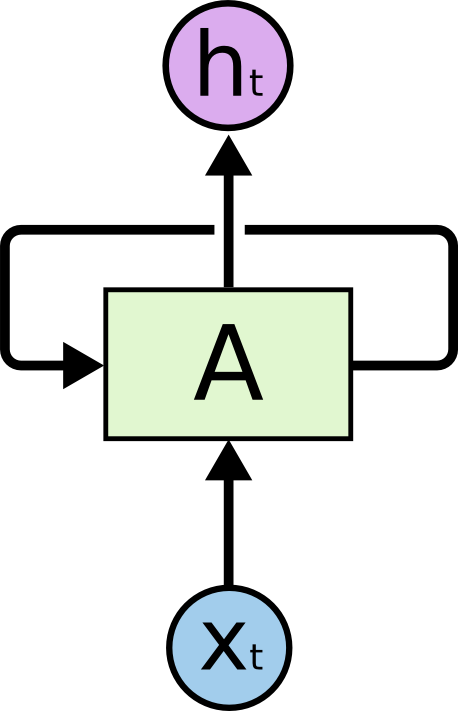
\includegraphics[scale=0.4]{./figs/rnn-rolled}
	\caption[A Rolled Recurrent Neural Networks]{Recurrent Neural Networks (RNNs) uses loops.}
	\label{fig:rnn-rolled}
\end{figure}

As it shown in \textbf{Figure \ref{fig:rnn-rolled}}, a selected neural network, $A$ takes the input $x_t$ and outputs the value of $h_t$. this might not show how data goes from one step to the next one in a same network until you unroll the loop and see chain architecture of recurrent neural networks that makes them the best choice for sequential data, \textbf{Figure \ref{fig:rnn-unrolled}}.

\begin{figure}[p]
	\centering
	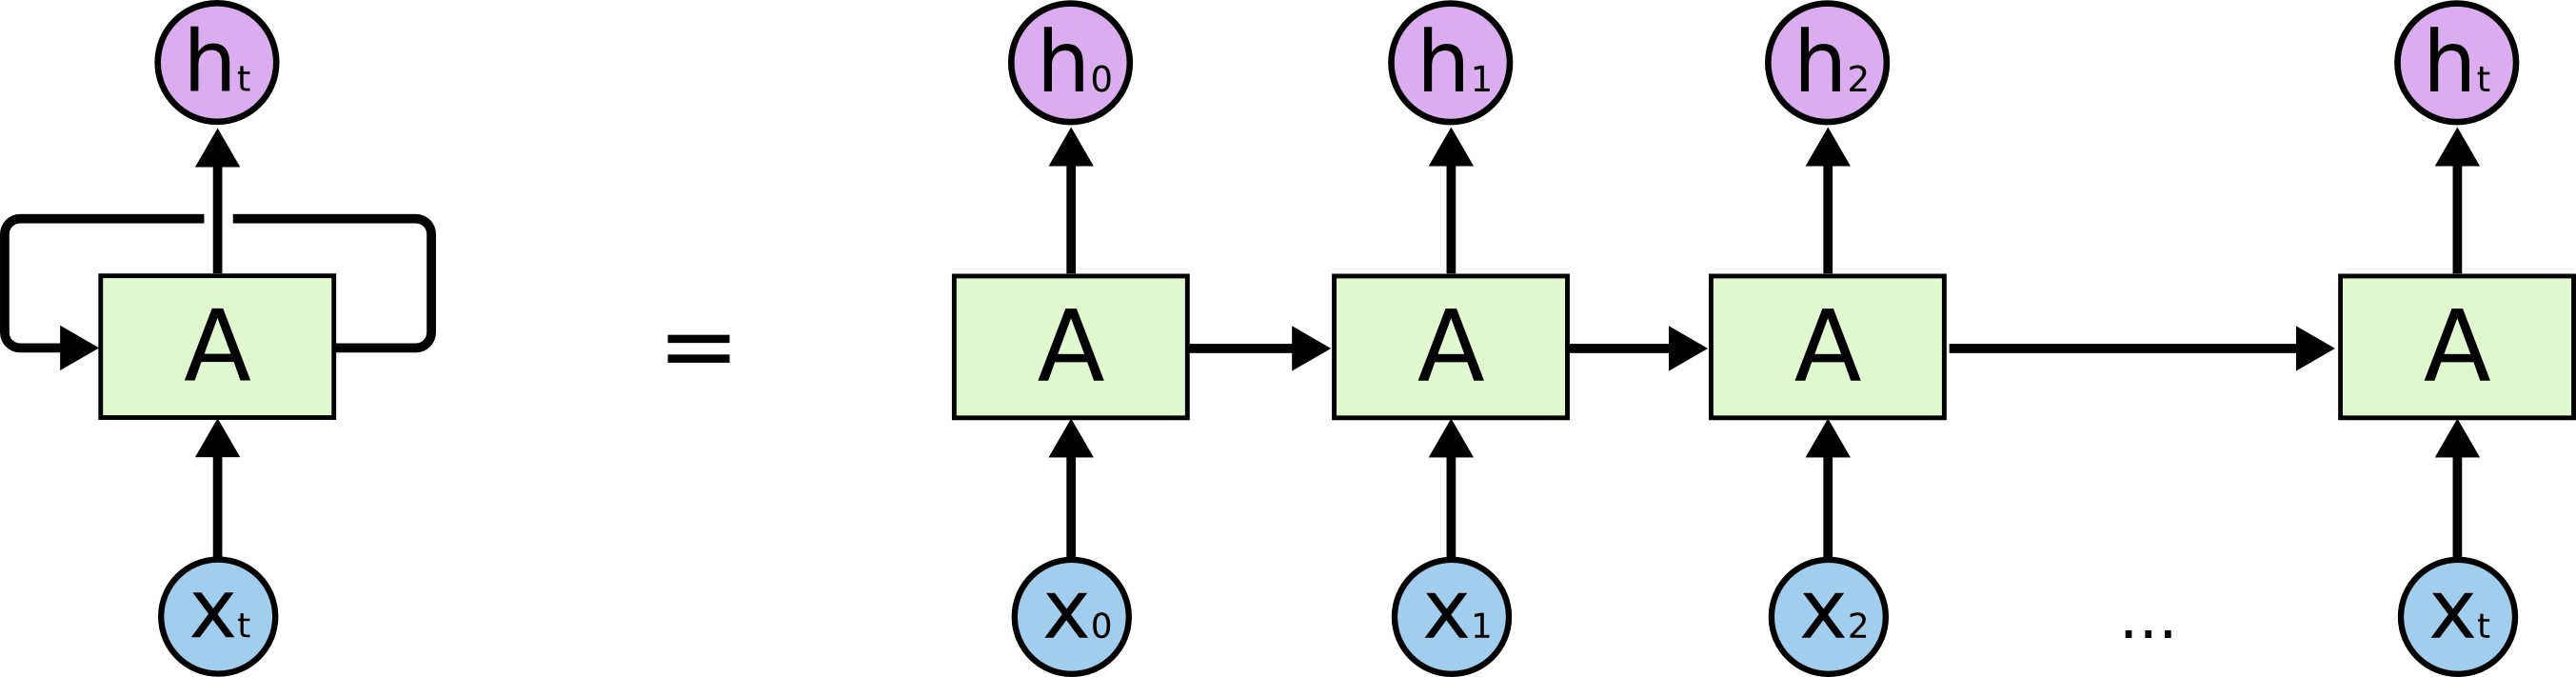
\includegraphics[scale=0.4]{./figs/rnn-unrolled}
	\caption[An Unrolled Recurrent Neural Networks]{An Unrolled Recurrent Neural Networks (RNNs).}
	\label{fig:rnn-unrolled}
\end{figure}

While RNNs is being used in variety of applications from language modeling to image captioning, the essential to all these achievement is the RNN-LSTMs \cite{Hochreiter1997}. An enhanced version of RNNs that outperforms better than the standard RNN.

\subsection{Model Confidence}
The model confidence has a critical role in different applications from early cancer detection in MRI scans, autonomous vehicles, and even simple image classification.
As an example, a trained model to distinguish dogs breeds,
it (hopefully) performs well with any given test photo of any dogs. But what if the model being tested by a cat photo which lies outside of the data distribution that this model was trained on.

These examples of \textit{out of distribution} test data can be extended to more serious cases like MRI scans or scenes that an autonomous vehicle model has not trained on before.
Other reasons that might cause uncertainty in data or model, like observed labels in data might be noisy or several models could fit the dataset which will cause uncertainty in model parameters.
Information on uncertainty also could help recognize whether the model is under-confident or falsely over-confident.

\section{Similar Works}
One similar approach is line search, where $\eta$ is a trained parameter that does line search along the gradient direction to give probabilistic interpretations to line search, while in this work the novel technique is to use a variational posterior with the reparametrization gradient.

Another similar technique is dynamic evaluation \cite{Mikolov2010}, which trains the RNN during evaluation steps of the model with a fixed learning rate. The drawback of this technique is that each update applied in this case is cumulative, and only uses previously seen data.

Finally, learning to optimise \cite{Li2016a} is also considered as similar work since it is learned and expected to produce better updates than the rest suggested by AdaGrad \cite{Duchi2011} or Adam \cite{Kingma2013a}. 

\section{State-of-the-Arts}
Adopting Bayesian methods to any neural networks has a vast background, with most common approximations having been tried.
\cite{Buntine1991} propose various maximum a posteriori schemes for neural networks, including an approximate posterior
centered at the mode.
\cite{Buntine1991} also suggest using second order derivatives in the prior to accelerate smoothness of the resulting NN.
\cite{Hinton1993} proposed using variational methods for compressing the weights of neural networks as a regulariser.
\cite{Hochreiter1995} suggest an MDL loss for single layer networks that penalises non-robust weights by means of an approximate penalty based upon perturbations of the weights on the outputs.
\cite{Mackay1995} investigated using the Laplace approximation for capturing the posterior of NNs.
\cite{Diggle} explored the use of hybrid Monte Carlo for training NNs; Notably, it has so far been difficult to apply these to the large sizes of networks.

More recently \cite{Graves2011} derived a variational inference scheme for NNs and
\cite{Blundell2015a} completed this with an update for the variance that is unbiased and simpler to compute.
\cite{Graves2016} derives a similar algorithm in the case of a mixture posterior.
Many researches have claimed that dropout \cite{Srivastava2014} and Gaussian dropout \cite{Wang2013} can be viewed as approximate variational inference schemes \cite{Gal2015}, \cite{Kingma2015}.
\cite{Gan2016} goes a step further and uses Monte Carlo dropout for LSTMs\footnote{One of the selected benchmark}.
Variational methods typically underestimate the uncertainty in the posterior, since they are mode seeking, depend to the Laplace approximation, whereas expectation propagation methods are mode averaging and almost tend to overestimate uncertainty.
Nevertheless, a few papers explored applying expectation propagation to NNs:
\cite{Soudry2014} derive a closed form approximate online expectation propagation algorithm, whereas \cite{Adams2015a} proposed using multiple passes of assumed density filtering (in combination with early stopping) attaining good performance on a number of small data sets.
\cite{Teh2015a} derive a distributed expectation propagation scheme with SGLD \cite{Welling2011} as an inner loop.
Others have also considered applying SGLD to neural networks \cite{Li2016a} and \cite{Gan2016} more recently used SGLD for LSTMs\footnote{One of the selected benchmark}.

\section{Research Gaps}
Adopting Bayes by Backprop (BBB) to Recurrent neural networks (RNNs), where the weight matrices of the RNN are drawn from a distribution could raise two questions:

\begin{enumerate}
	\item What stage to sample the parameters of the RNNs?
	\item How to weight the contrubution of KL regularisation?
\end{enumerate}

\section{Technique: Backprop Through Time}
\label{sec:bptt}

As illustrated in \ref{fig:rnn-rolled}, the core of an recurrent neural networks (RNNs), $f$, is a neural network that maps the RNN state at step $t$, $s_t$ and an input observation $x_t$ to a new RNN state $s_{t+1}$, $f: (s_t, x_t) \mapsto s_{t+1}$.

For comparison, an LSTM-powered RNN core \cite{Hochreiter1997} has a state $s_t = (c_t, h_t)$ where $c$ is an internal core state and $h$ is the exposed state. Intermediate gates modulate the effect of the inputs on the outputs, gates like the input gate $i_t$, forget gate $f_t$ and output gate $o_t$. The correlation between the inputs, outputs and internal gates of an LSTM cell can be explained as:

\begin{align*}
i_t &= \sigma(W_i [x_t, h_{t-1}]^T + b_i), \\
f_t &= \sigma(W_f [x_t, h_{t-1}]^T + b_f), \\
c_t &= f_t c_{t-1} + i_t \tanh(W_c [x_t, h_{t-1}] + b_c), \\
o_t &= \sigma(W_o [x_t, h_{t-1}]^T + b_o), \\
h_t &= o_t \tanh(c_t),
\end{align*}

In the above statement, $W_i$ ($b_i$), $W_f$ ($b_f$), $W_c$ ($b_c$) and $W_o$ ($b_o$) are the weights (biases) that are affecting the input gate, forget gate, cell update, and output gate accordingly.

An RNN can be trained on a sequence of $T$ using backpropagation through time where the RNN is unrolled $T$ times like a feed-forward network.
Which can be achieve with forming the feed-forward network with inputs
$x_1, x_2, \dots, x_T$ and initial state $s_0$:

\begin{align}
s_1 &= f(s_0, x_1), \nonumber \\
s_2 &= f(s_1, x_2), \nonumber \\
&\dots \nonumber \\
\label{eq:unroll}
s_T &= f(s_{T-1}, x_T), 
\end{align}

where $s_T$ is the total length (final state) of the RNN.
Referring to the unrolled RNN for $T$ steps as in \eqref{eq:unroll} by $s_{1:T} = F_T(x_{1:T}, s_0)$,
where $x_{1:T}$ is the sequence of input vectors and $s_{1:T}$ is the sequence of corresponding states. However, the truncated version of the algorithm can be seen as taking $s_0$ as the last state of the previous batch, $s_T$.

This RNN parameters are trained in the same way as a feed-forward neural network and a loss is applied to the states $s_{1:T}$ of the RNN, and then backpropagation is being used to update the weights of the trained network.
Since the weights in each of the unrolled step are shared, each weight of the RNN core receives $T$ gradient contributions when the it is unrolled for $T$ steps.

\section{Chapter Summary}
This chapter reviewed the general concept of Recurrent Neural Networks (RNNs) and described the enhanced version of RNN-LSTMs. The model confidence of NNs has been discussed with different application examples. 

Moreover, similar approaches have been studied and the long history of applying Bayes to NNs described to justify the state-of-the-art. The proposed technique, backprop through time, has been extensively described.